\documentclass[a4paper,10pt]{article}
%-----------------------------------------------------------
\usepackage[top=0.75in, bottom=0.75in, left=0.55in, right=0.85in]{geometry}
\usepackage{graphicx}
\usepackage{url}
\usepackage{palatino}
\usepackage{tabularx}
\fontfamily{Calibri}
\selectfont

\usepackage[T1]{fontenc}
\usepackage
%[ansinew]
[utf8]
{inputenc}

\usepackage{color}
\definecolor{mygrey}{gray}{0.75}
\textheight=9.75in
\raggedbottom

\setlength{\tabcolsep}{0in}
\newcommand{\isep}{-2 pt}
\newcommand{\lsep}{-0.5cm}
\newcommand{\psep}{-0.6cm}
\renewcommand{\labelitemii}{$\circ$}

\pagestyle{empty}
%------------------------------------------------------------
%Custom commands
\newcommand{\resitem}[1]{\item #1 \vspace{-2pt}}
\newcommand{\resheading}[1]{{\small \colorbox{mygrey}{\begin{minipage}{0.975\textwidth}{\textbf{#1 \vphantom{p\^{E}}}}\end{minipage}}}}
\newcommand{\ressubheading}[3]{
\begin{tabular*}{6.62in}{l @{\extracolsep{\fill}} r}
	\textsc{{\textbf{#1}}} & \textsc{\textit{[#2]}} \\
\end{tabular*}\vspace{-8pt}}
%-----------------------------------------------------------

\begin{document}
\hspace{0.5cm}\\[-0.2cm]
\begin{flushright}
\large
\textbf{Mukesh P} \\
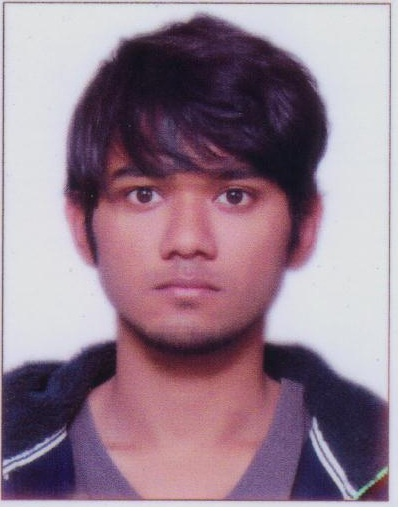
\includegraphics[width = 30mm]{a.jpg}
\end{flushright}

\indent \resheading{\textbf{CONTACT INFORMATION} }\\[\lsep]
\\ \\

\indent\begin{tabular}{@{}p{3.5in}p{3.5in}}
Plot no. 12, Road no. 14, &{Phone No.:} +91-9869365330 \\ 
Sector 12, New Panvel,	&  {Email-id:}mukesh85tek@gmail.com \\
Navi Mumbai, Maharashtra - 410206   \\
\end{tabular}

\indent\resheading{\textbf{CAREER OBJECTIVE} }\\[\lsep]
\\ \\
\indent To be a part of an organization that provides an atmosphere of mutual growth and benefits, where I can \indent show  my talent and potential.


\indent\resheading{\textbf{EDUCATION} }\\[\lsep]
\\ \\
\indent \begin{tabular}{ l @{\hskip 0.15in} l @{\hskip 0.15in} l @{\hskip 0.15in} l @{\hskip 0.15in} l}
	\hline
	\textbf{Examination} & \textbf{University} & \textbf{Institute} & \textbf{Year} & \textbf{CPI} \\
	\hline
	10th Board & CBSE & D.A.V. Public School & 2010 & 9.8 \\
	\hline
	12th Board & CBSE & Shiv Jyoti School & 2012 & 81\% \\
	\hline
	B.E. & Mumbai University & Fr. Rodrigues Institute of technology, Vashi & 2016 & 7.7\\
	\hline
\end{tabular}
\\ \\

\resheading{\textbf{PROJECTS} }\\[\lsep]
\\ \\
\begin{enumerate}
		\item COLLEGE INTRANET
		\subitem Objective: To make sharing of data easier between students and teachers. \\
		\indent \indent Languages and tools: Android, Java Swing.
		
		\item NETWORK PERFORMANCE MONITOR
		\subitem Objective: To calculate the throughput of a system when different types of connection are established.
		\indent \indent Languages and tools: Java Swing.
\end{enumerate}

\resheading{\textbf{TRAINING AND INTERNSHIP} }\\[\lsep]
\\ \\
\begin{itemize}
	\item
\end{itemize}

\resheading{\textbf{RESEARCH PUBLICATIONS} }\\[\lsep]
\\ \\
\begin{enumerate}
	\item
\end{enumerate}


\resheading{\textbf{TECHNICAL SKILLS} }\\[\lsep]
\\ \\
\begin{itemize}
	\item
\end{itemize}

\resheading{\textbf{SOFT SKILLS} }\\[\lsep]
\\ \\
\begin{enumerate}
	\item
\end{enumerate}

\resheading{\textbf{EXTRA CURRICULAR} }\\[\lsep]
\\ \\
\begin{itemize}
	\item
\end{itemize}

\resheading{\textbf{CO-CURRICULAR} }\\[\lsep]
\\ \\
\begin{enumerate}
	\item
\end{enumerate}

\resheading{\textbf{PERSONAL INFORMATION} }\\[\lsep]
\\ \\


\resheading{\textbf{REFERENCE} }\\[\lsep]
\\ \\

\resheading{\textbf{DECLARATION} }\\[\lsep]
\\ \\


\resheading{\textbf{DATE} }\\[\lsep]
\\ \\

\end{document}

